
\section{Iteration 1: Interactive Environment}
\label{sec:iteration_no1}

This is the first iteration of the prototyping phase.
The main goal is to get a \ac{MVP} running, what exactly this entails,
how it was achieved, how this relates to our \nameref{suggested_architecture}
and what the results of this iteration are, will be discussed in the following sections.


\subsection{Milestones and Goals}

The main goal of this iteration is to have an Arkouda environment running on the cluster,
which is accessible through a Jupyter client running on a local machine.

The milestones to be reached in order to achieve this goal are as follows:

\begin{enumerate}
    \item \textbf{Verification} While there is an existing installation running on the cluster,
          it has been running unattended for roughly a year and was originally intended for a different purpose.
          Therefore the first step is to verify that the installation is still operational and that the environment is still functional.
    \item \textbf{Deployment of Jupyter} The next step is to deploy a Jupyter server on the cluster,
          which is able to access the Arkouda environment. In order to do this a custom container
          image will need to be created, to run alongside the existing Arkouda environment.
    \item \textbf{Access from Local Machine} The final step is to make the service as low barrier as possible,
          by making it accessible from a local device.

\end{enumerate}

\subsection{Implementation}

\subsubsection{Verification}

Considering that the original installation was done as an experiment and has been running unattended for a year,
and has survived a hardware change and a resizing of the cluster, it is still operational.
One issue that was discovered during later steps was that during a final reformating of the repository,
the name variable of an \ac{RBAC} role was changed, which caused subsequent redeployment to fail,
but which was quickly resolved after the issue was identified\footcite{joneckerthFixingErroneousRBAC}.

\subsubsection{Deployment of Jupyter}

While there exist many ready made images for Jupyter,
the way the Arkouda client needs to be installed and configured requires a custom image to be created.
This is due to the fact that the Arkouda client library is not available through any standard package manager,
but needs to be installed from source\footcite{arkouda-repoArkoudaPydocSetup},
the same goes for the \textit{Chapel} compiler Arkouda is built on\footcite{chapel-lang.orgBuildingChapelChapel}.
Making the users do this manually would be a waste of time and compute resources.
Additionally in order to make the connection to the Arkouda environment,
\textit{IPython Kernel} needs to have access to current connection information at initiation and runtime.

\textbf{Image: }

The first step was to create this custom image,
the foundational image for this is the image provided by the \textit{Chapel} project\footcite{chapelChapelProfileDockera},
as it already contains a whole precompiled version of Chapel.
This is important as the Arkouda client library needs to use the binaries provided by Chapel,
in order to create the necessary shared objects for the Python bindings\footcite{arkouda-repoArkoudaPydocSetup}.
One thing which was not clear was, wether the Chapel binaries where still
needed after the shared objects were created, as our version only needs to act as a client.
After the chapel binaries and the Arkouda client library were installed,
the single user notebook server was installed and the \textit{IPython} kernel was
extended to load the required modules and establish the connection to the Arkouda environment as
well as to terminate the connection when the kernel is shut down.

\textbf{Deployment: }

In oder to get this custom image to work on the cluster,
a deployment script was created which has access to the internal network of the Arkouda Namespace and the
connection information needed to establish the connection to the Arkouda endpoint.
The container was then pushed to the clusters \gls{registry} and deployed to the cluster.

\textbf{Testing: }
\label{testing_iteration_no1}

To see wether the whole integration works the setup was
tested with scripts provided by the Arkouda project for demonstration purposes\footcite{arkouda-repoBearsRUsArkoudaNotebooksPlace}.
Unfortunately the system did not work as expected, the program terminating with the indication that the
requests of the client where not being answered by the server.
Due to no error messages being produced by the server,
the assumption being that the connection, going through all layers of the Kubernetes network stack,
was suddenly being dropped silently. After thorough investigation it was discovered that the
issue was instead caused by a bug in the Arkouda \textit{argsort} function causing a silent
crash of the process, when the function was called on a string array\footcite{hokiegeek2CommitsBearsRUsArkouda}.
For the initial prototype it was worked around by \gls{monkey patching} the function to use the \textit{NumPy} implementation
instead when the input is a string array.
This is not an ideal solution, as the \textit{NumPy} implementation is not distributed and therefore not as performant as the Arkouda implementation.
But this will get address in the next iteration, where the performance of the environment will be improved.
With this workaround in place the scripts provided by the Arkouda project where able to run successfully,
and the connection to the Arkouda environment was established and stable for the duration of the test.
More thorough testing in form of a benchmark for each of the operations will be done in the next iteration at \autoref{sec:iteration_no2}.


\subsubsection{Access from Local Machine}
The final step is to make the service accessible from a local device,
with the knowledge gained from the previous research, this was a simple task.
The Jupyter container was exposed to the outside world (the corporate intranet)
through a \textit{NodePort} service, which is now accessible from any device on the network.
In order to prevent unauthorized access, as the service is not secured by default,
additionally a password was set for the Jupyter server.

\begin{figure}[!ht]
    \centering
    \scalebox{0.32}{
        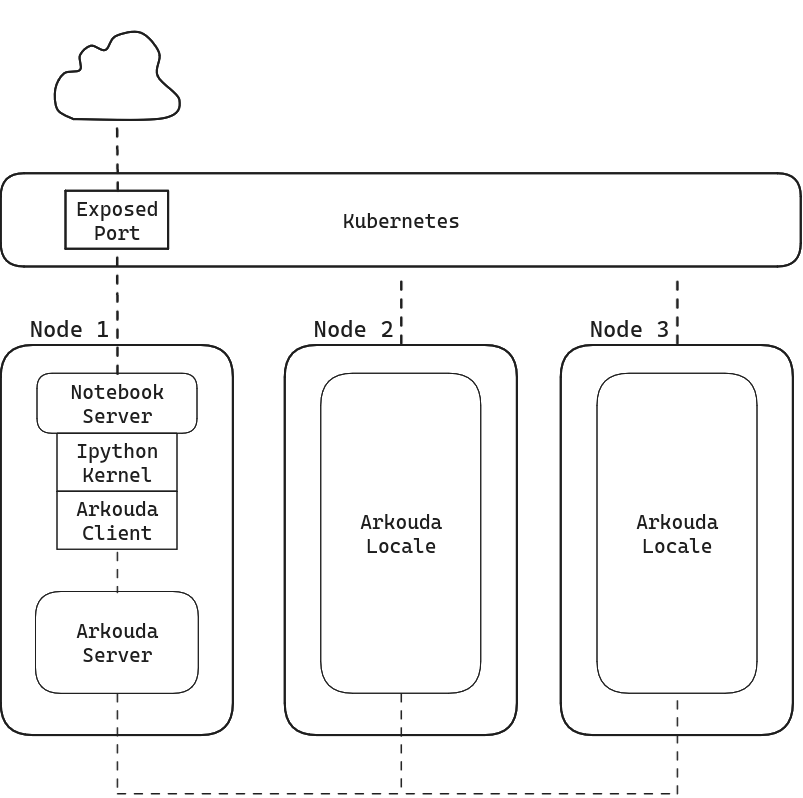
\includegraphics{./graphics/Jupyter-setup.png}
    }
    \vspace{0.6cm}
    \caption{ High Level Overview of the Jupyter Setup}
    \label{fig:juptyer_setup}
\end{figure}


In diagram \ref{fig:juptyer_setup} above is shown how the setup is structured, most importantly the Jupyter container is
the only container which is exposed to the outside world, the Arkouda container is only accessible from the Jupyter container.
Which itself connects to the \textit{Arkouda} Server only through a node internal network connection.
Each of the Ipython kernels has its own independent connection to the Arkouda server,
which is established at the start of the kernel and terminated at the end of the kernel.

Currently this system is completely ephemeral, as neither the Jupyter container nor the \textit{Arkouda}
\ac{GASNet} domain are being persisted.


\subsection{Evaluation of Results}


The Goal of this iteration was the creation of a \ac{MVP} of an interactive Arkouda environment
running on a multi node compute cluster, accessible through a Jupyter client.
While some issues where encountered during the implementation, the goal was successfully achieved.
The Arkouda environment is now accessible from any device on the corporate intranet,
and the connection to the Arkouda environment is stable and easily usable.

During the implementation some original assumptions made during the research a  nd the \Nameref{suggested_architecture}
but showed to be infeasible or incorrect and had to be adjusted.

% arkouda being young and promising might be a good idea to invest more time into it, especially since it still has some bugs which need to be fixed.

While using Chapel as the base for the high performance computing has shown to be a good choice,
the choice of using Arkouda to increase the ease of use for python developers has shown
that it is still quite young in comparison to long established libraries like \textit{NumPy},
and sometimes lacks \ac{QoL} features, like a simple pip based installation or a more verbose error handling.
But as it is unrivaled in the area of python based distributed computing on large scale data\footcite{ronaghanSqueezingPerformanceOut2020},
it is a promising library to invest more time into.

% original proposition was to use the arkouda container as a base layer, which was not possible due to ...
While there exits a container image to be used as an Arkouda client, which was intended
to be used as a base layer for the Jupyter container,
is build on the basis of an \ac{SMP} Chapel compilation.
If the Chapel binaries need to be replaced anyhow,
there is no reason not to use the right Chapel image from the start,
and building everything on top of that our self.

% Removing the reference to something that was not implemented
% % As of right now no autoscaling of the service
% As of right now there is only a single deployment of the services running on the cluster,
% with the express purpose of having more than one user at a time, utilizing 
% the cluster to its full potential, the service should be autoscaled.
% But in order to first have a comparable baseline, this was out of scope for this iteration,
% and as we are planning to use a topology aware deployment strategy, this should be addressed in \ref{sec:iteration_no3}.

% Fazit
\textbf{Conclusion:}

The goal of this iteration was to create a \ac{MVP} of an interactive Arkouda environment,
which is accessible from a local device. This goal was successfully achieved.
The environment is now accessible from any device on the corporate intranet,
and the connection to the Arkouda environment is stable and easily usable.

The initial assumptions made during the research phase and the \nameref{suggested_architecture},
where addressed and corrected during the implementation phase.
And during the implementation some new issues where discovered,
such as an issue with a function in the Arkouda library which will need to be addressed.
The next iteration will focus on improving the performance of the environment,
as during the testing the opportunity for improvement was discovered.

\pagebreak
